\documentclass[tikz,border=6pt]{standalone}

\usepackage[T1]{fontenc}
\usepackage{lmodern}
\usepackage{xcolor}
\usetikzlibrary{shapes,arrows,positioning,calc}

\begin{document}
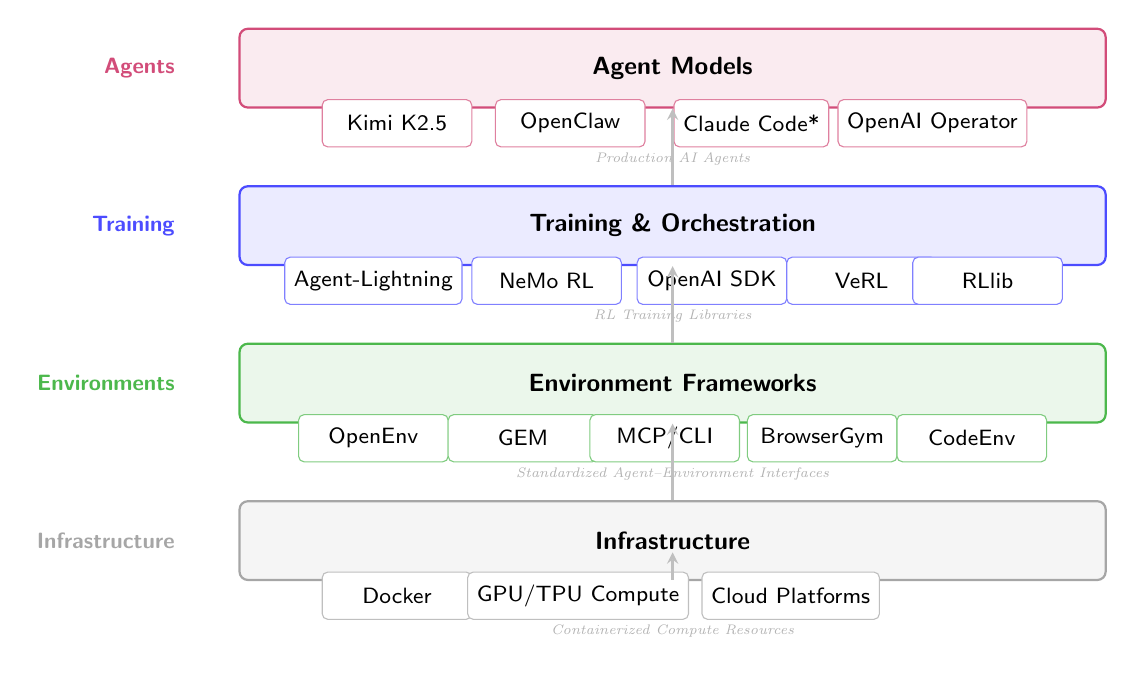
\begin{tikzpicture}[
    layer/.style={rectangle, draw=#1!70, fill=#1!8, minimum width=11cm, minimum height=1.0cm, align=center, font=\small\sffamily, thick, rounded corners=3pt},
    item/.style={rectangle, draw=#1!50, fill=white, minimum width=1.9cm, minimum height=0.6cm, align=center, font=\footnotesize\sffamily, rounded corners=2pt, thin},
    lbl/.style={font=\footnotesize\sffamily\bfseries, text=#1!70, anchor=east},
    sublbl/.style={font=\tiny\itshape, text=gray!60}
]
% Infrastructure
\node[layer=gray] (infra) at (0,0) {\textbf{Infrastructure}};
\node[item=gray] at (-3.5,-0.7) {Docker};
\node[item=gray] at (-1.2,-0.7) {GPU/TPU Compute};
\node[item=gray] at (1.5,-0.7) {Cloud Platforms};
\node[sublbl] at (0,-1.15) {Containerized Compute Resources};

% Environment Frameworks
\node[layer=green!60!black] (envf) at (0,2.0) {\textbf{Environment Frameworks}};
\node[item=green!60!black] at (-3.8,1.3) {OpenEnv};
\node[item=green!60!black] at (-1.9,1.3) {GEM};
\node[item=green!60!black] at (-0.1,1.3) {MCP/CLI};
\node[item=green!60!black] at (1.9,1.3) {BrowserGym};
\node[item=green!60!black] at (3.8,1.3) {CodeEnv};
\node[sublbl] at (0,0.85) {Standardized Agent--Environment Interfaces};

% Training
\node[layer=blue] (train) at (0,4.0) {\textbf{Training \& Orchestration}};
\node[item=blue] at (-3.8,3.3) {Agent-Lightning};
\node[item=blue] at (-1.6,3.3) {NeMo RL};
\node[item=blue] at (0.5,3.3) {OpenAI SDK};
\node[item=blue] at (2.4,3.3) {VeRL};
\node[item=blue] at (4.0,3.3) {RLlib};
\node[sublbl] at (0,2.85) {RL Training Libraries};

% Agent Models
\node[layer=purple] (agent) at (0,6.0) {\textbf{Agent Models}};
\node[item=purple] at (-3.5,5.3) {Kimi K2.5};
\node[item=purple] at (-1.3,5.3) {OpenClaw};
\node[item=purple] at (1.0,5.3) {Claude Code*};
\node[item=purple] at (3.3,5.3) {OpenAI Operator};
\node[sublbl] at (0,4.85) {Production AI Agents};

% Layer labels on left
\node[lbl=gray] at (-6.2,0) {Infrastructure};
\node[lbl=green!60!black] at (-6.2,2.0) {Environments};
\node[lbl=blue] at (-6.2,4.0) {Training};
\node[lbl=purple] at (-6.2,6.0) {Agents};

% Vertical arrows
\draw[->, >=stealth, thick, gray!50] (0,-0.5) -- (0,-0.15);
\draw[->, >=stealth, thick, gray!50] (infra.north) -- (envf.south);
\draw[->, >=stealth, thick, gray!50] (envf.north) -- (train.south);
\draw[->, >=stealth, thick, gray!50] (train.north) -- (agent.south);
\end{tikzpicture}
\end{document}